%#########################################################################
\chapter{Oscilaciones}
\label{cha:oscillations}

El concepto de oscilación es ampliamente usado en ciencia y se aplica para
cualquier cantidad que presente fluctuaciones o perturbaciones en función 
del tiempo, ya sean periódicas o no. En este capítulo se presentan algunos
ejemplos de oscilaciones para sistemas mecánicos y electromagnéticos, que 
a pesar de su simplicidad, permiten ahondar en los detalles físicos de este
tipo de fenómenos.

\

La forma estándar de abordar un problema en una disciplina científica 
consiste en el estudio de situaciones ideales y muy particulares para llegar 
luego, usando refinamientos y consideraciones posteriores, a descripciones 
realistas y más generales. Por este motivo se comienza con demostraciones 
computacionales aplicadas a sistemas ideales, como el péndulo simple, el 
sistema masa resorte, etc. En demostraciones siguientes se abordarán 
aspectos cada vez más complejos de estos sistemas.
%#########################################################################



\
%*************************************************************************
\section{Demostración 1: Péndulo Simple Ideal}
\label{sec:DEMO2_01}
\rule{14cm}{0.5mm}

Como primer caso se aborda el péndulo simple. Este consiste en un sistema
de una masa $m$ con dimensión despreciable y bajo la acción de la 
gravedad $\bds g$, además pende de una cuerda tensa de longitud $l$ y sujeta
en un punto fijo. A partir de la figura \ref{fig:simple_pendulum}, la 
ecuación de movimiento está dada por


%.........................................................................
%Movement equation
\eq{eq:simple_pendulum}
{m\dtot{^2\bds r}{t^2} = m\bds g + \bds T}
%.........................................................................

\newpage
%.........................................................................
%Simple Pendulum
\begin{figure}[htbp]
	\centering
	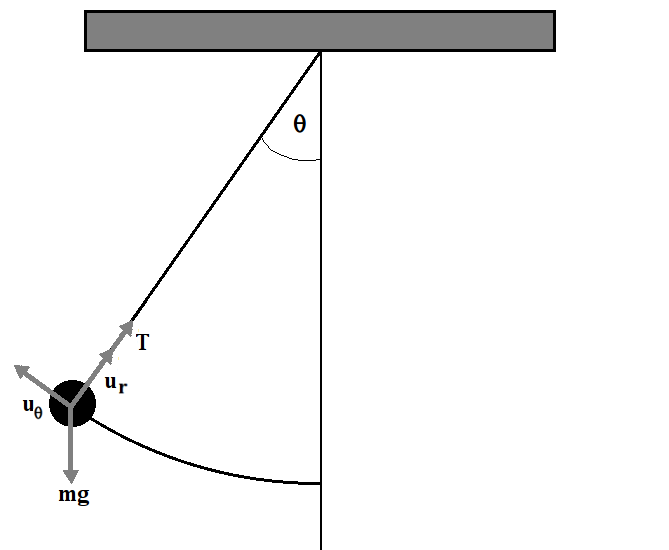
\includegraphics[width=0.50\textwidth]
	{./pictures/simple_pendulum.png}

	\caption{\small{Péndulo simple bajo la acción del campo gravitacional.}}
	
	\label{fig:simple_pendulum}
\end{figure}
%.........................................................................


En coordenadas polares se obtiene


%.........................................................................
%Movement equations
\begin{eqnarray}
\label{eq:simple_pendulum_1}
ml\dot \theta^2 &=& T - mg \cos \theta \\
\label{eq:simple_pendulum_2}
ml\ddot \theta &=& -mg \sin \theta
\end{eqnarray}
%.........................................................................


Como primera demostración computacional de este capítulo se solucionará el 
movimiento del péndulo simple a partir de las ecuaciones 
\ref{eq:simple_pendulum_1} y \ref{eq:simple_pendulum_2}. Para esto se 
asumirá que la amplitud de oscilación del péndulo es pequeña de tal forma 
que $\theta \approx \sin \theta$ y $\cos \theta \approx 1$, obteniendo


%.........................................................................
%Simplified equation
\eq{eq:simplified_pendulum}
{\ddot \theta = - \frac{g}{l} \theta}
%.........................................................................


Usando un ansatz de la forma $\theta(t) = e^{\lambda t}$ se llega a la
solución


%.........................................................................
%Approximate solution
\eq{eq:pendulum_solution}
{ \theta(t) = \theta_0 \sin ( \omega_0 t + \delta ) }
%.........................................................................
donde $\theta_0$ y $\delta$ son la amplitud y la fase respectivamente y 
constituyen las condiciones iniciales. La frecuencia $\omega_0$ está 
definida por 


%.........................................................................
%Frequancy
\eq{eq:freq_pedulum}
{ \omega_0 = \sqrt{ \frac{g}{l} } }
%.........................................................................

\

En el siguiente script de \python se grafica esta solución para diferentes
valores de la amplitud y la fase.

\newpage
%ccccccccccccccccccccccccccccccccccccccccccccccccccccccccccccccccccccccccc
%DEMO 2_01
\begin{listing}[style=python]
#!/usr/bin/env python
#==========================================================
# DEMOSTRACION 1
# Grafica de soluciones aproximadas del pendulo simple
#==========================================================
import numpy as np
import matplotlib.pylab as plt

#Solucion
def Theta(t):
    theta = theta0*np.sin( omega0*t + delta )
    return theta
    
#Gravedad
g = 9.8
#Longitud
l = 1
#Frecuencia
omega0 = np.sqrt( g/l )
#Tiempos
tiempo = np.arange( 0, 10, 0.1 )
    
#SOLUCION 1
#Amplitud
theta0 = 0.05
#Fase
delta = 0.0
#Grafica
plt.plot( tiempo, Theta(tiempo), label='solucion 1' )

#SOLUCION 2
#Amplitud
theta0 = 0.05
#Fase
delta = np.pi
#Grafica
plt.plot( tiempo, Theta(tiempo), label='solucion 2' )

#SOLUCION 3
#Amplitud
theta0 = 0.1
#Fase
delta = 0.0
#Grafica
plt.plot( tiempo, Theta(tiempo), label='solucion 3' )

plt.legend()
plt.show()
\end{listing}
%ccccccccccccccccccccccccccccccccccccccccccccccccccccccccccccccccccccccccc


El resultado que se obtiene es


%.........................................................................
%Simple Pendulum
\begin{figure}[htbp]
	\centering
	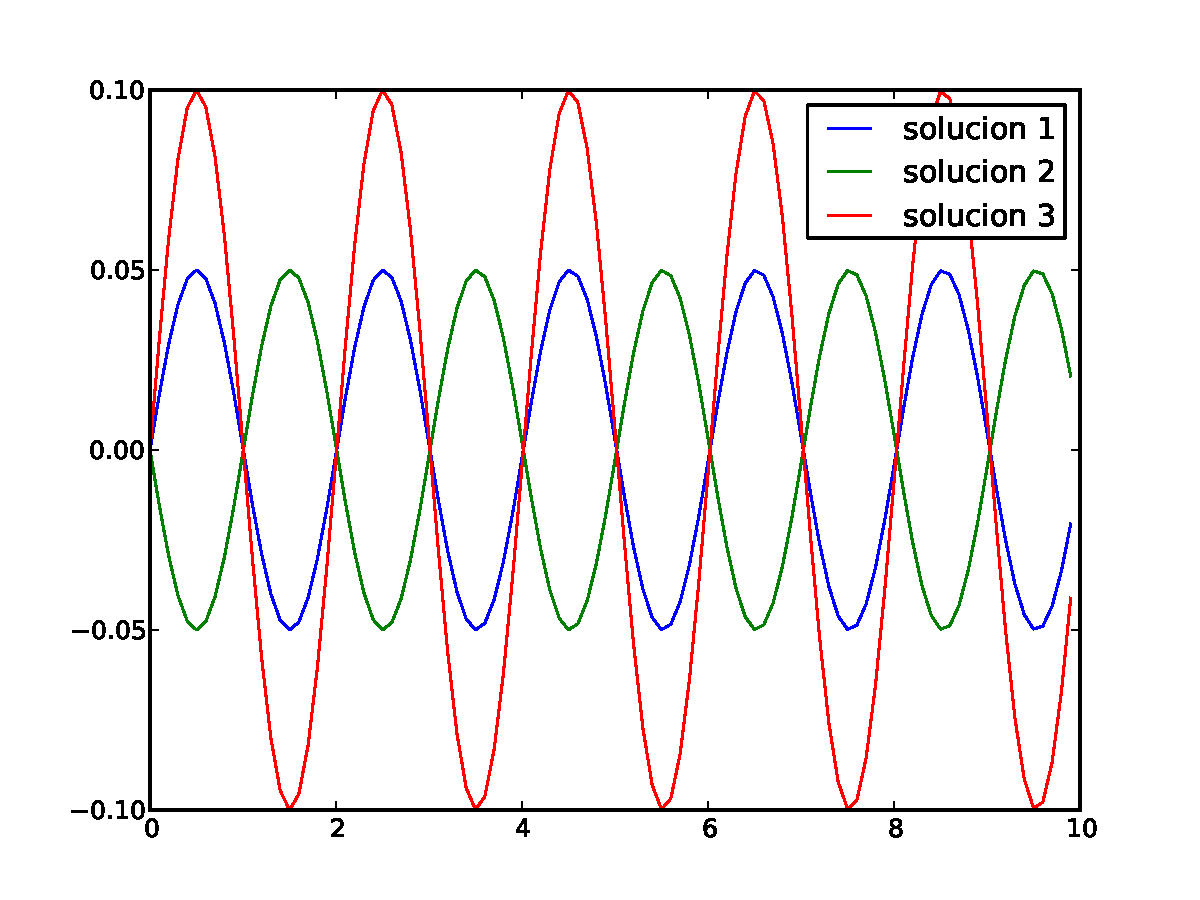
\includegraphics[width=0.8\textwidth]
	{./pictures/demo2_01.pdf}

	\caption{\small{Soluciones aproximadas obtenidas para el péndulo simple.}}
	
	\label{fig:approx_pedulum}
\end{figure}
%.........................................................................


En lo siguiente se explica cada porción de código.


%ccccccccccccccccccccccccccccccccccccccccccccccccccccccccccccccccccccccccc
%DEMO 2_01
\begin{listing}[style=python, numbers = none]
import numpy as np
import matplotlib.pylab as plt
\end{listing}
%ccccccccccccccccccccccccccccccccccccccccccccccccccccccccccccccccccccccccc
Esto corresponde al cargado de las librerías \numpy, bajo el alias de np y
\matplotlib bajo el alias de plt, ambas son necesarias para el desarrollo 
de todo el código.


%ccccccccccccccccccccccccccccccccccccccccccccccccccccccccccccccccccccccccc
%DEMO 2_01
\begin{listing}[style=python, numbers = none]
#Solucion
def Theta(t):
    theta = theta0*np.sin( omega0*t + delta )
    return theta
\end{listing}
%ccccccccccccccccccccccccccccccccccccccccccccccccccccccccccccccccccccccccc
En este parte se define la solución obtenida en la ecuación 
\ref{eq:pendulum_solution} para cualquier tiempo dado. Las funciones 
matemáticas estándar, tales como exponencial, logaritmo, trigonométricas, 
hiperbólicas, etc. Son accedidas desde el módulo \numpy como \texttt{np.sin},
\texttt{np.sinh}, \texttt{np.exp}, \texttt{np.log}, etc.


%ccccccccccccccccccccccccccccccccccccccccccccccccccccccccccccccccccccccccc
%DEMO 2_01
\begin{listing}[style=python, numbers = none]
#Gravedad
g = 9.8
#Longitud
l = 1
#Frecuencia
omega0 = np.sqrt( g/l )
#Tiempos
tiempo = np.arange( 0, 10, 0.1 )
\end{listing}
%ccccccccccccccccccccccccccccccccccccccccccccccccccccccccccccccccccccccccc
Se define la gravedad, la longitud de la cuerda (en metros), la frecuencia
de oscilación y finalmente, usando la función \texttt{arange} de la librería
\numpy, se cons\-truye un arreglo de tiempos donde es evaluada la solución, de 
0 a 10 segundos con saltos de 0.1.


%ccccccccccccccccccccccccccccccccccccccccccccccccccccccccccccccccccccccccc
%DEMO 2_01
\begin{listing}[style=python, numbers = none]
#SOLUCION 1
#Amplitud
theta0 = 0.05
#Fase
delta = 0.0
#Grafica
plt.plot( tiempo, Theta(tiempo), label='solucion 1' )
\end{listing}
%ccccccccccccccccccccccccccccccccccccccccccccccccccccccccccccccccccccccccc
La primera solución es obtenida para una amplitud de $\theta_0 = 0.05$ 
radianes y una fase $\delta = 0$. La última línea corresponde a la 
construcción de la gráfica de la solución. Para esto se usa la función 
\texttt{plot} de la librería \matplotlib. El primer argumento corresponde
a los datos asociados al eje x, en este caso \texttt{tiempo}, mientras el
segundo argumento son los datos asociados al eje y, en este caso la solución
evaluada en el tiempo, es decir \texttt{Theta(tiempo)}. El argumento 
\texttt{label} indica el nombre que tendrá la solución en la gráfica final,
esto se denomina etiqueta de la función.


%ccccccccccccccccccccccccccccccccccccccccccccccccccccccccccccccccccccccccc
%DEMO 2_01
\begin{listing}[style=python, numbers = none]
plt.legend()
plt.show()
\end{listing}
%ccccccccccccccccccccccccccccccccccccccccccccccccccccccccccccccccccccccccc
Finalmente se termina el script con la función \texttt{legend}, la cual 
muestra en pantalla las etiquetas puestas a cada gráfica. Y la función 
\texttt{show} que muestra en pantalla todas las soluciones.

\rule{14cm}{0.5mm}
%*************************************************************************



\
%*************************************************************************
\section{Demostración 2: Solución Exacta del Péndulo}
\label{sec:DEMO2_02}
\rule{14cm}{0.5mm}

La solución propuesta en la demostración anterior está basada en la 
aproximación de pequeñas oscilaciones, para la cual $\sin \theta \approx 
\theta$ y $\cos \theta \approx 1$, aún así, a medida que el movimiento sea
de mayor amplitud, esta aproximación deja de ser válida y se la solución 
general debe obtenerse directamente de las ecuaciones 
\ref{eq:simple_pendulum_1} y \ref{eq:simple_pendulum_2}

\

Una forma conveniente de reescribir las ecuaciones de movimiento es derivando
\ref{eq:simple_pendulum_1} respecto al tiempo e introduciendo la ecuación
\ref{eq:simple_pendulum_2}


%.........................................................................
%Tension
\begin{eqnarray}
\nonumber
\dot T &=& \dot \theta \pr{ 2ml\ddot \theta - mg\sin \theta } \\
\nonumber
\dot T &=& -\dot \theta \pr{ 2mg\sin \theta + mg\sin \theta } \\
\label{eq:new_tension}
\dot T &=& -3\dot \theta mg\sin \theta
\end{eqnarray}
%.........................................................................


Definiendo la velocidad angular $\omega = \dot \theta$, el sistema de 
ecuaciones originales junto con la ecuación \ref{eq:new_tension} queda


%.........................................................................
%Equations linealized
\begin{eqnarray}
\label{eq:Dtheta}
\dot \theta &=& \omega \\
\label{eq:Domega}
\dot \omega &=& -\frac{g}{l}\sin \theta \\
\label{eq:Dtension}
\dot T &=& -3\omega mg\sin \theta
\end{eqnarray}
%.........................................................................


Esta forma se denomina sistema de ecuaciones diferenciales lineales y es 
esencial para la solución exacta a partir de algoritmos de integración 
numérica.

\

Las condiciones iniciales para la solución aproximada son completamente 
determinadas a partir de la fase $\delta$ y la amplitud $\theta_0$. En el 
caso de la solución exacta es necesario suministrar tres condiciones para
cada una de las variables de las ecuaciones \ref{eq:Dtheta} - 
\ref{eq:Dtension}, es decir, la posición angular inicial del péndulo 
$\theta_{t_0}$, la velocidad angular inicial $\omega_{t_0}$ y la tensión
inicial $T_{t_0}$. Aún así, la tensión inicial depende de las otras dos 
condiciones a través de la ecuación \ref{eq:simple_pendulum_1}


%.........................................................................
%T0_equation
\eq{eq:initial_tension}
{T_{t_0} = ml\omega_{t_0}^2 + mg \cos \theta_{t_0}}
%.........................................................................


En esta demostración se calcularán ambas soluciones para un péndulo con 
condiciones iniciales fijadas. La solución numérica se realiza a partir del
la rutina de integración numérica \texttt{odeint} del módulo \texttt{integrate}
del paquete \scipy.


%ccccccccccccccccccccccccccccccccccccccccccccccccccccccccccccccccccccccccc
%DEMO 2_02
\begin{listing}[style=python]
#!/usr/bin/env python
#==========================================================
# DEMOSTRACION 2
# Comparacion de solucion completa y aproximada para el 
# pendulo simple
#==========================================================
import numpy as np
import matplotlib.pylab as plt
import scipy.integrate as integ

#Solucion aproximada
def Theta(t):
    theta = theta0*np.sin( omega0*t + delta )
    return theta

#Ecuaciones de movimiento
def dF(Y, t):
    #Valor anterior de theta
    theta = Y[0]
    #Valor anterior de omega
    omega = Y[1]
    #Valor anterior de la tension
    tension = Y[2]
    #Derivada de theta
    Dtheta = omega
    #Derivada de omega
    Domega = -g*np.sin( theta )/l
    #Derivada de la tension
    Dtension = -3*omega*m*g*np.sin( theta )
    return (Dtheta, Domega, Dtension)
    
#Gravedad
g = 9.8
#Longitud
l = 1
#Masa
m = 1
#Frecuencia
omega0 = np.sqrt( g/l )
#Tiempos
tiempo = np.arange( 0, 10, 0.01 )
    
#SOLUCION APROXIMADA
#Amplitud
theta0 = np.pi/4
#Fase
delta = np.pi/2.
#Grafica
plt.plot(tiempo, Theta(tiempo), label='solucion aproximada')

#SOLUCION NUMERICA
#Angulo inicial
theta_t0 = np.pi/4
#Velocidad angular inicial
omega_t0 = 0.0
#Tension inicial
tension_t0 = m*l*omega_t0**2 + m*g*np.cos( theta_t0 )
#Condiciones iniciales
cond_ini = ( theta_t0, omega_t0, tension_t0 )
#Solucion numerica
theta_t, omega_t, tension_t = np.transpose( 
integ.odeint( dF, cond_ini, tiempo ) )
#Grafica
plt.plot( tiempo, theta_t, label='solucion numerica' )

plt.legend()
plt.show()
\end{listing}
%ccccccccccccccccccccccccccccccccccccccccccccccccccccccccccccccccccccccccc

\

Para ambas soluciones se ha asumido una amplitud de $\theta_0 = 45^o = 
\pi/4$ y las condiciones iniciales son definidas de tal forma que el 
péndulo sea soltado desde su máxima amplitud. En el caso de la solución 
aproximada, esto implica una amplitud $\theta_0 = \pi/4$ y una fase de 
$\delta = \pi/2$. Para la solución aproximada, las condiciones equivalentes 
son $\theta_{t_0} = \pi/4$ y $\omega_{t_0} = 0$. El resultado de la 
integración para 10 segundos es mostrado en la figura 
\ref{fig:numeric_pedulum}.

\

Cambiando la amplitud inicial a un valor $\theta = 10^o \approx 0.17$ 
ambas soluciones son muy similares, indicando el rango de la validez de 
la aproximación inicial. El resultado para 10 segundos es mostrado en la 
figura \ref{fig:small_pedulum}.


%.........................................................................
%Simple Pendulum Exact solution
\begin{figure}[htbp]
	\centering
	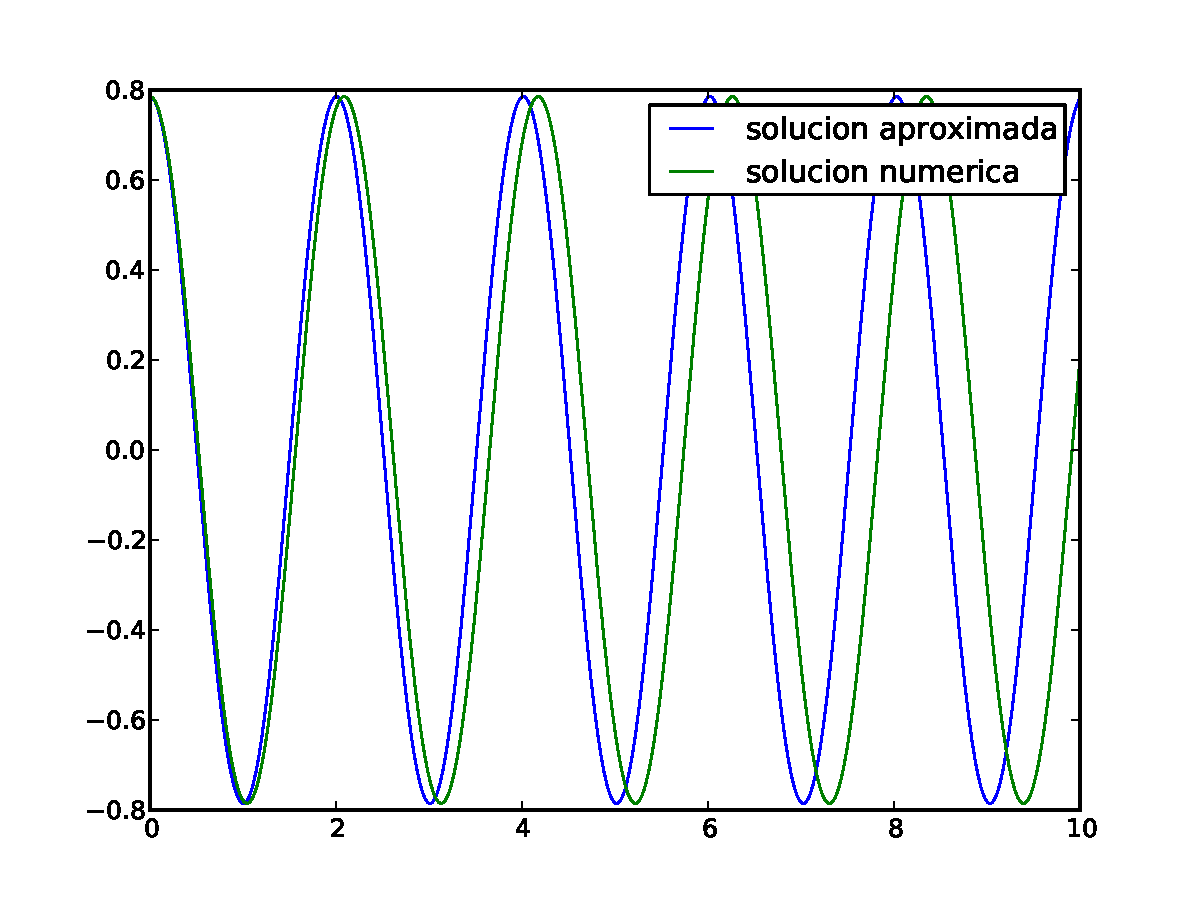
\includegraphics[width=0.80\textwidth]
	{./pictures/demo2_02.pdf}

	\caption{\small{Comparación entre la solución exacta numérica y la 
	solución aproximada. Debido a la mayor amplitud de oscilación, la 
	aproximación de pequeñas oscilaciones deja de ser válida y difiere 
	considerablemente de la solución real.}}
	
	\label{fig:numeric_pedulum}
\end{figure}
%.........................................................................


%.........................................................................
%Simple Pendulum Exact solution
\begin{figure}[htbp]
	\centering
	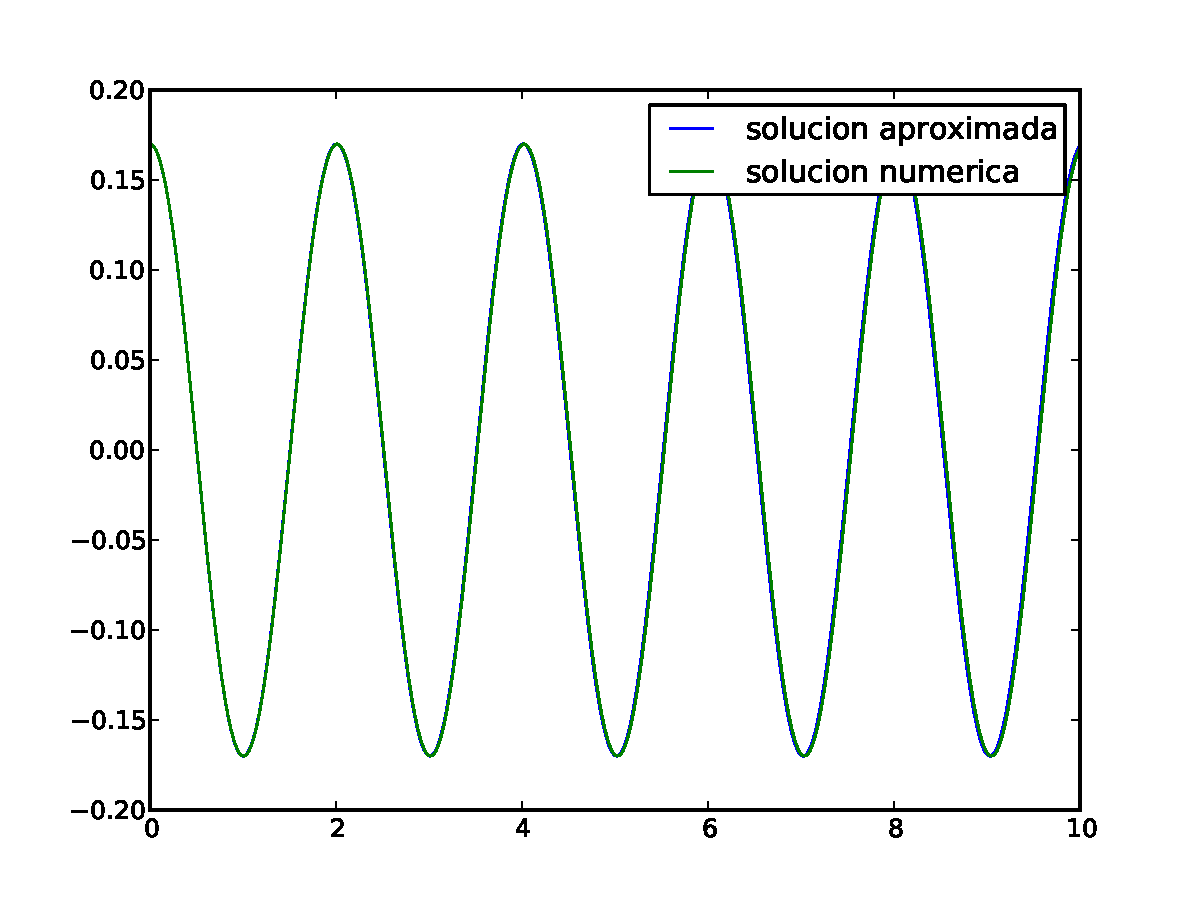
\includegraphics[width=0.80\textwidth]
	{./pictures/demo2_02(02).pdf}

	\caption{\small{Comparación entre la solución exacta numérica y la 
	solución aproximada. Para pequeñas amplitudes ambas soluciones son
	muy similares.}}
	
	\label{fig:small_pedulum}
\end{figure}
%.........................................................................
\newpage

A continuación se explican las nuevas partes introducidas en el código en 
comparación con la demostración 1.


%ccccccccccccccccccccccccccccccccccccccccccccccccccccccccccccccccccccccccc
%DEMO 2_02
\begin{listing}[style=python, numbers = none]
import scipy.integrate as integ
\end{listing}
%ccccccccccccccccccccccccccccccccccccccccccccccccccccccccccccccccccccccccc
Esto corresponde al cargado del módulo \texttt{integrate} de \scipy bajo el
alias de \texttt{integ} para las funcionalidades de integración numérica.


%ccccccccccccccccccccccccccccccccccccccccccccccccccccccccccccccccccccccccc
%DEMO 2_02
\begin{listing}[style=python, numbers = none]
#Ecuaciones de movimiento
def dF(Y, t):
    #Valor anterior de theta
    theta = Y[0]
    #Valor anterior de omega
    omega = Y[1]
    #Valor anterior de la tension
    tension = Y[2]
    #Derivada de theta
    Dtheta = omega
    #Derivada de omega
    Domega = -g*np.sin( theta )/l
    #Derivada de la tension
    Dtension = -3*omega*m*g*np.sin( theta )
    return (Dtheta, Domega, Dtension)
\end{listing}
%ccccccccccccccccccccccccccccccccccccccccccccccccccccccccccccccccccccccccc
Se define la función que contiene las derivadas de cada una de las 
variables del sistema, acorde al sistema \ref{eq:Dtheta} - \ref{eq:Dtension}.
\texttt{Y} es un arreglo que contiene las variables $\theta$, $\omega$ y $T$
evaluadas en el tiempo anterior respectivamente y finalmente el argumento 
\texttt{t} es el tiempo actual.


%ccccccccccccccccccccccccccccccccccccccccccccccccccccccccccccccccccccccccc
%DEMO 2_02
\begin{listing}[style=python, numbers = none]
#SOLUCION NUMERICA
#Angulo inicial
theta_t0 = np.pi/4
#Velocidad angular inicial
omega_t0 = 0.0
#Tension inicial
tension_t0 = m*l*omega_t0**2 + m*g*np.cos( theta_t0 )
#Condiciones iniciales
cond_ini = ( theta_t0, omega_t0, tension_t0 )
#Solucion numerica
theta_t, omega_t, tension_t = np.transpose( 
integ.odeint( dF, cond_ini, tiempo ) )
#Grafica
plt.plot( tiempo, theta_t, label='solucion numerica' )
\end{listing}
%ccccccccccccccccccccccccccccccccccccccccccccccccccccccccccccccccccccccccc
En esta parte se realiza la integración de la solución exacta del péndulo 
simple. Se dan las condiciones iniciales para el ángulo y la velocidad 
angular inicial, para la tensión se usa la ecuación \ref{eq:initial_tension}.
Luego, en un arreglo \texttt{cond\_ini} se dan las tres condiciones para 
luego llamar la función \texttt{integ.odeint}. Esta tiene como primer 
argumento la función \texttt{dF} con las ecuaciones de movimiento del 
sistema, segundo argumento el arreglo de condiciones iniciales y 
como tercero el arreglo de tiempo donde se desea evaluar la solución.
Finalmente se grafica la solución.

\rule{14cm}{0.5mm}
%*************************************************************************



\
%*************************************************************************
\section{Demostración 3: Sistema de Péndulos Acoplados}
\label{sec:DEMO2_03}
\rule{14cm}{0.5mm}


En esta demostración se abordarán aspectos más complejos de computación,
donde se comenzará a realizar animaciones y representaciones 3D a partir
de la librería \mayavi. Como tercera demostración se plantea entonces un 
sistema acoplado de 4 péndulos simples de diferente longitud tal como se 
muestra en la figura \ref{fig:four_pendulums}.


%.........................................................................
%Acopled Pendulum
\begin{figure}[htbp]
	\centering
	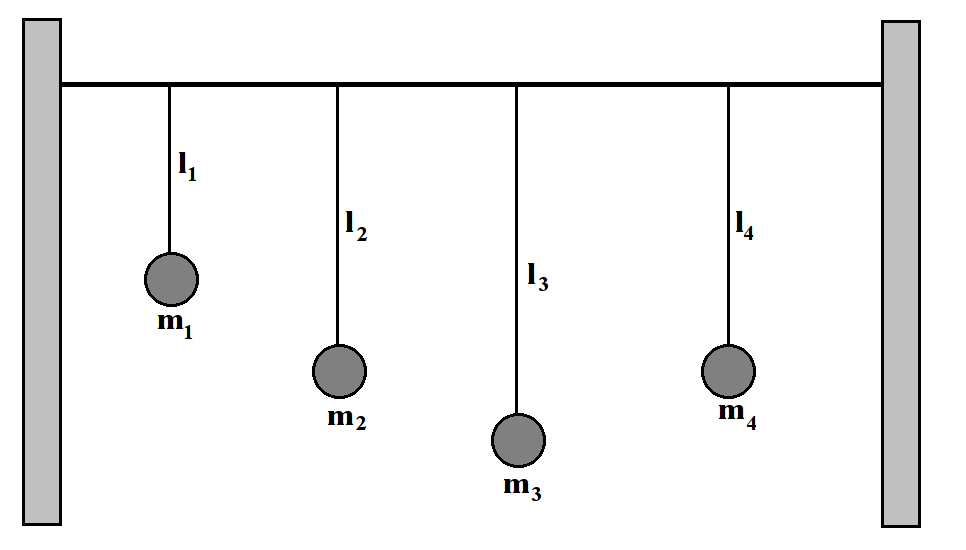
\includegraphics[width=0.70\textwidth]
	{./pictures/acopled_pendulum.png}

	\caption{\small{Sistema de 4 péndulos acoplados.}}
	
	\label{fig:four_pendulums}
\end{figure}
%.........................................................................


Todos los péndulos son de dimensión despreciable de tal forma que pueden 
ser considerados puntuales, además todos penden de una cuerda tensionada
y no de un cuerpo rígido debido a que la cuerda actúa como agente de 
acoplamiento en el sistema, permitiendo el intercambio de energía entre los
péndulos.


Para modelar el término de acoplamiento entre los péndulos se supondrá que
cada péndulo solo interactúa de forma apreciable con sus vecinos más 
cercanos y que la fuerza de interacción solo actúa en la dirección 
horizontal determinada por el eje \textit{x}, siendo proporcional a la 
solución de los vecinos próximos. Teniendo esto en consideración, a 
ecuación de movimiento para el i-ésimo péndulo es


%.........................................................................
%Acopled Pendulum
\begin{figure}[htbp]
	\centering
	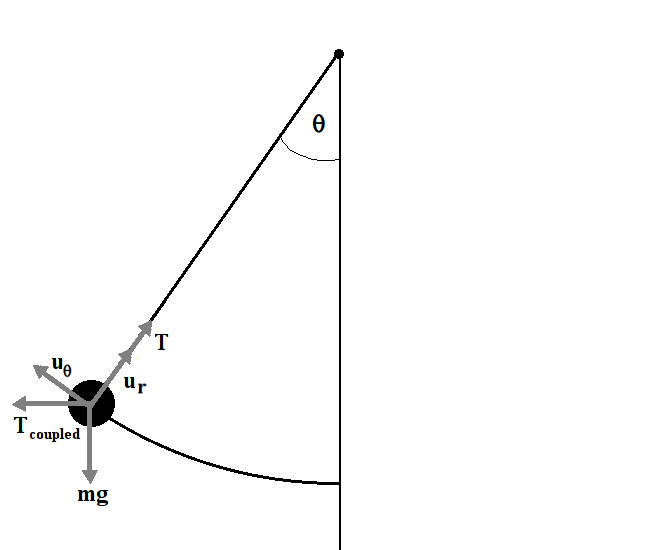
\includegraphics[width=0.60\textwidth]
	{./pictures/acopled_individual_pendulum.png}

	\caption{\small{i-ésimo péndulo del sistema acoplado. La fuerza de 
	acoplamiento actúa en el eje horizontal.}}
	
	\label{fig:i_pendulum}
\end{figure}
%.........................................................................


%.........................................................................
%Movement equation of individual acopled pendulum
\eq{eq:individual_pendulum}
{m\dtot{^2\bds r_i}{t^2} = m\bds g + \bds T_i + \
\bds T_{c,i-1} + \bds T_{c,i+1}}
%.........................................................................
donde $\bds T_{c,i+1}$ y $\bds T_{c,i-1}$ son los términos de acoplamiento
asociados a los péndulos vecinos, en caso de no existir uno de los vecinos,
el término es nulo. Por simplicidad y sin pérdida de generalidad se asumirán 
péndulos de masas iguales. Finalmente, con el objetivo de cuantificar la 
fuerza de acoplamiento, se usará el peso de los péndulos de tal forma que 


%.........................................................................
%Acopled force
\eq{eq:acopled_force}
{\bds T_{c,j} = f m g \theta_j(t) \bds i}
%.........................................................................
con $\theta_j(t)$ la solución del péndulo j y $f$ un factor que indica la 
magnitud de la fuerza de acoplamiento en unidades $mg$. En principio, este
factor depende de la tensión de la cuerda principal de la cual penden los
péndulos, pero por simplicidad se tomará como un parámetro libre de tal 
forma que $f \ll 1$. 

\newpage

Descomponiendo las ecuaciones de movimiento en coordenadas polares del 
i-ésimo péndulo tal como se hizo para el péndulo simple en la demostración 
1 \ref{sec:DEMO2_01} se llega a 


%.........................................................................
%Movement equations
\begin{eqnarray}
\label{eq:indv_pendulum_1}
ml\dot \theta_i^2 &=& T_i - mg \cos \theta_i - 
fmg\pr{ \theta_{i-1} + \theta_{i+1} }\sin \theta_i \\
\label{eq:indv_pendulum_2}
ml\ddot \theta_i &=& -mg \sin \theta_i +  
fmg\pr{ \theta_{i-1} + \theta_{i+1} }\cos{\theta_i}
\end{eqnarray}
%.........................................................................


Al igual que la demostración 2 \ref{sec:DEMO2_02}, no se realizará la 
aproximación de pequeñas oscilaciones y las ecuaciones serán resueltas de
forma numérica. Es necesario entonces llevar las ecuaciones \ref{eq:indv_pendulum_1}
\ref{eq:indv_pendulum_2} a una sistema de ecuaciones diferenciales lineales,
para esto se deriva la ecuación \ref{eq:indv_pendulum_1} respecto al tiempo
y se reemplaza el termino en $\ddot \theta_i$ por la ecuación 
\ref{eq:indv_pendulum_2}.


%.........................................................................
%Tension acopled
\begin{eqnarray}
\nonumber
\dot T_i &=& \dot \theta_i \cor{ 2ml\ddot \theta_i - mg\sin \theta_i + 
fmg\pr{\theta_{i-1} + \theta_{i+1}}\cos{\theta_i}} \\
\nonumber
& &+ fmg\pr{\dot \theta_{i-1} + 
\dot \theta_{i+1}}\sin{\theta_i} \\
\nonumber
\dot T_i &=& 3\dot \theta_i\cor{ fmg \pr{\theta_{i-1} + 
\theta_{i+1}}\cos{\theta_i} - mg \sin \theta_i  } \\
\label{eq:new_acopled_tension}
&& + fmg\pr{\dot \theta_{i-1} + \dot\theta_{i+1}}\sin{\theta_i}
\end{eqnarray}
%.........................................................................


Introduciendo de nuevo la definición de velocidad angular $\omega_i = 
\dot \theta_i$ se obtiene


%.........................................................................
%Equations linealized of acopled pendulums
\begin{eqnarray}
\label{eq:Dthetai}
\dot \theta_i &=& \omega_i \\
\label{eq:Domegai}
\dot \omega_i &=& -\frac{g}{l}\sin \theta_i +  
f\frac{g}{l}\pr{ \theta_{i-1} + \theta_{i+1} }\cos{\theta_i} \\
\nonumber
\dot T_i &=& 3\omega_i\cor{ fmg \pr{\theta_{i-1} + 
\theta_{i+1}}\cos{\theta_i} - mg \sin \theta_i } \\
\label{eq:Dtensioni}
&& + fmg\pr{\omega_{i-1} + \omega_{i+1}}\sin{\theta_i}
\end{eqnarray}
%.........................................................................


Se llega entonces a un sistema de $3\times 4 = 12$ ecuaciones diferenciales 
acopladas. Note que haciendo el parámetro de acoplamiento nulo $f = 0$ se 
llega de nuevo al péndulo simple de la demostración 2.

\

El conjunto de condiciones iniciales se definirá de tal forma que el 
sistema presente resonancia entre dos péndulos, para esto los tres primeros
péndulos partirán del reposo mientras el cuarto péndulo comenzará oscilando
con una amplitud de $\theta_4(t=0) = 45^o = \pi /4 \mbox{ rad}$. La 
longitud de los péndulos serán respectivamente $l_1 = 1$ m, $l_2 = 2$ m, 
$l_3 = 3$ m y $l_4 = 2$ m, de esta forma se garantiza una resonancia 
entre los péndulos 2 y 4. El estudiante puede modificar estas condiciones
en los códigos y así recrear las situaciones que desee.

\

Esta tercera demostración se dividirá en dos diferentes códigos, el primer
script realizará la integración numérica de los péndulos y guardará las 
soluciones en un archivo de datos (\texttt{demo2\_03\_1.py}), el segundo 
script cargará estos archivos de datos y realizará la animación 3D del 
sistema (\texttt{demo2\_03\_2.py}) \footnote{Recuerde que puede descargar 
los códigos originales del repositorio oficial del curso en 
\url{https://github.com/sbustamante/Computacional-OscilacionesOndas/tree/master/codigos}}.


%ccccccccccccccccccccccccccccccccccccccccccccccccccccccccccccccccccccccccc
%DEMO 2_03_1
\begin{listing}[style=python]
#!/usr/bin/env python
#==========================================================
# DEMOSTRACION 3: Parte 1
# Solucion numerica de 4 pendulos simples acoplados
#==========================================================
from __future__ import division
import numpy as np
import matplotlib.pylab as plt
import scipy.integrate as integ

#Ecuaciones de movimiento
def dF(Y, t):
    #Valor anterior de theta pendulo 1
    theta1 = Y[0]
    #Valor anterior de omega pendulo 1
    omega1 = Y[1]
    #Valor anterior de la tension pendulo 1
    tension1 = Y[2]
    
    #Valor anterior de theta pendulo 2
    theta2 = Y[3]
    #Valor anterior de omega pendulo 2
    omega2 = Y[4]
    #Valor anterior de la tension pendulo 2
    tension2 = Y[5]
    
    #Valor anterior de theta pendulo 3
    theta3 = Y[6]
    #Valor anterior de omega pendulo 3
    omega3 = Y[7]
    #Valor anterior de la tension pendulo 3
    tension3 = Y[8]
    
    #Valor anterior de theta pendulo 4
    theta4 = Y[9]
    #Valor anterior de omega pendulo 4
    omega4 = Y[10]
    #Valor anterior de la tension pendulo 4
    tension4 = Y[11]
    
    #Derivada de theta pendulo 1
    Dtheta1 = omega1
    #Derivada de omega pendulo 1
    Domega1 = -(g/l1)*np.sin( theta1 ) + \
    f*(g/l1)*( theta2 )*np.cos( theta1 )
    #Derivada de la tension pendulo 1
    Dtension1 = -3*omega1*(-m*g*np.sin( theta1 ) + \
    f*m*g*( theta2 )*np.cos( theta1 )) + \
    f*m*g*( omega2 )*np.sin( theta1 )
    
    #Derivada de theta pendulo 2
    Dtheta2 = omega2
    #Derivada de omega pendulo 2
    Domega2 = -(g/l2)*np.sin( theta2 ) + \
    f*(g/l2)*( theta1 + theta3 )*np.cos( theta2 )
    #Derivada de la tension pendulo 2
    Dtension2 = -3*omega2*(-m*g*np.sin( theta2 ) + \
    f*m*g*( theta1 + theta3 )*np.cos( theta2 )) + \
    f*m*g*( omega1 + omega3 )*np.sin( theta2 )
    
    #Derivada de theta pendulo 3
    Dtheta3 = omega3
    #Derivada de omega pendulo 3
    Domega3 = -(g/l3)*np.sin( theta3 ) + \
    f*(g/l3)*( theta2 + theta4 )*np.cos( theta3 )
    #Derivada de la tension pendulo 3
    Dtension3 = -3*omega3*(-m*g*np.sin( theta3 ) + \
    f*m*g*( theta2 + theta4 )*np.cos( theta3 )) + \
    f*m*g*( omega2 + omega4 )*np.sin( theta3 )
    
    #Derivada de theta pendulo 4
    Dtheta4 = omega4
    #Derivada de omega pendulo 4
    Domega4 = -(g/l4)*np.sin( theta4 ) + \
    f*(g/l4)*( theta3 )*np.cos( theta4 )
    #Derivada de la tension pendulo 4
    Dtension4 = -3*omega4*(-m*g*np.sin( theta4 ) + \
    f*m*g*( theta3 )*np.cos( theta4 )) + \
    f*m*g*( omega3 )*np.sin( theta4 )
    
    return (Dtheta1, Domega1, Dtension1, \
    Dtheta2, Domega2, Dtension2, \
    Dtheta3, Domega3, Dtension3, \
    Dtheta4, Domega4, Dtension4)
    
#Gravedad
g = 9.8
#Masa de todos los pendulos
m = 1.
#Longitud pendulo 1
l1 = 1.0
#Longitud pendulo 2
l2 = 2.0
#Longitud pendulo 3
l3 = 3.0
#Longitud pendulo 4
l4 = 2.0
#Factor de acoplamiento 
f = 0.1
#Tiempos
tiempo = np.arange( 0, 200, 0.1 )
    

#SOLUCION NUMERICA
#Condicion inicial pendulo 1
#Angulo inicial
theta1_t0 = 0.0
#Velocidad angular inicial
omega1_t0 = 0.0
#Tension inicial
tension1_t0 = m*l1*omega1_t0**2 + m*g*np.cos( theta1_t0 )

#Condicion inicial pendulo 2
#Angulo inicial
theta2_t0 = 0.0
#Velocidad angular inicial
omega2_t0 = 0.0
#Tension inicial
tension2_t0 = m*l2*omega2_t0**2 + m*g*np.cos( theta2_t0 )

#Condicion inicial pendulo 3
#Angulo inicial
theta3_t0 = 0.0
#Velocidad angular inicial
omega3_t0 = 0.0
#Tension inicial
tension3_t0 = m*l3*omega3_t0**2 + m*g*np.cos( theta3_t0 )

#Condicion inicial pendulo 4
#Angulo inicial
theta4_t0 = np.pi/4
#Velocidad angular inicial
omega4_t0 = 0.0
#Tension inicial
tension4_t0 = m*l3*omega3_t0**2 + m*g*np.cos( theta3_t0 )

#Condiciones iniciales de todos los pendulos
cond_ini = ( theta1_t0, omega1_t0, tension1_t0, \
theta2_t0, omega2_t0, tension2_t0,\
theta3_t0, omega3_t0, tension3_t0,
theta4_t0, omega4_t0, tension4_t0)
#Solucion numerica de todos los pendulos
theta1_t, omega1_t, tension1_t, \
theta2_t, omega2_t, tension2_t, \
theta3_t, omega3_t, tension3_t, \
theta4_t, omega4_t, tension4_t = \
np.transpose( integ.odeint( dF, cond_ini, tiempo ) )

#Guardado de resultados en archivo externo
datos = np.transpose((tiempo, theta1_t, theta2_t, \
theta3_t, theta4_t))
np.savetxt( 'amplitudes.txt', datos )

#Grafica de las soluciones
plt.plot( tiempo, theta1_t, label = 'pendulo 1', \
color='red', linewidth = 2 )
plt.plot( tiempo, theta2_t, label = 'pendulo 2', \
color='blue', linewidth = 2 )
plt.plot( tiempo, theta3_t, label = 'pendulo 3', \
color='green', linewidth = 2 )
plt.plot( tiempo, theta4_t, label = 'pendulo 4', \
color='black', linewidth = 2 )

#Formato de grafica
plt.title('Soluciones de pendulos acoplados')
plt.xlabel('tiempo')
plt.ylabel('Angulo oscilacion [rad]')
plt.grid()
plt.legend()
plt.show()
\end{listing}
%ccccccccccccccccccccccccccccccccccccccccccccccccccccccccccccccccccccccccc


Una vez corrido el programa se debe obtener el archivo \texttt{amplitudes.txt} 
con las soluciones angulares, y la siguiente figura 


%.........................................................................
%Acopled Pendulums Exact solution
\begin{figure}[htbp]
	\centering
	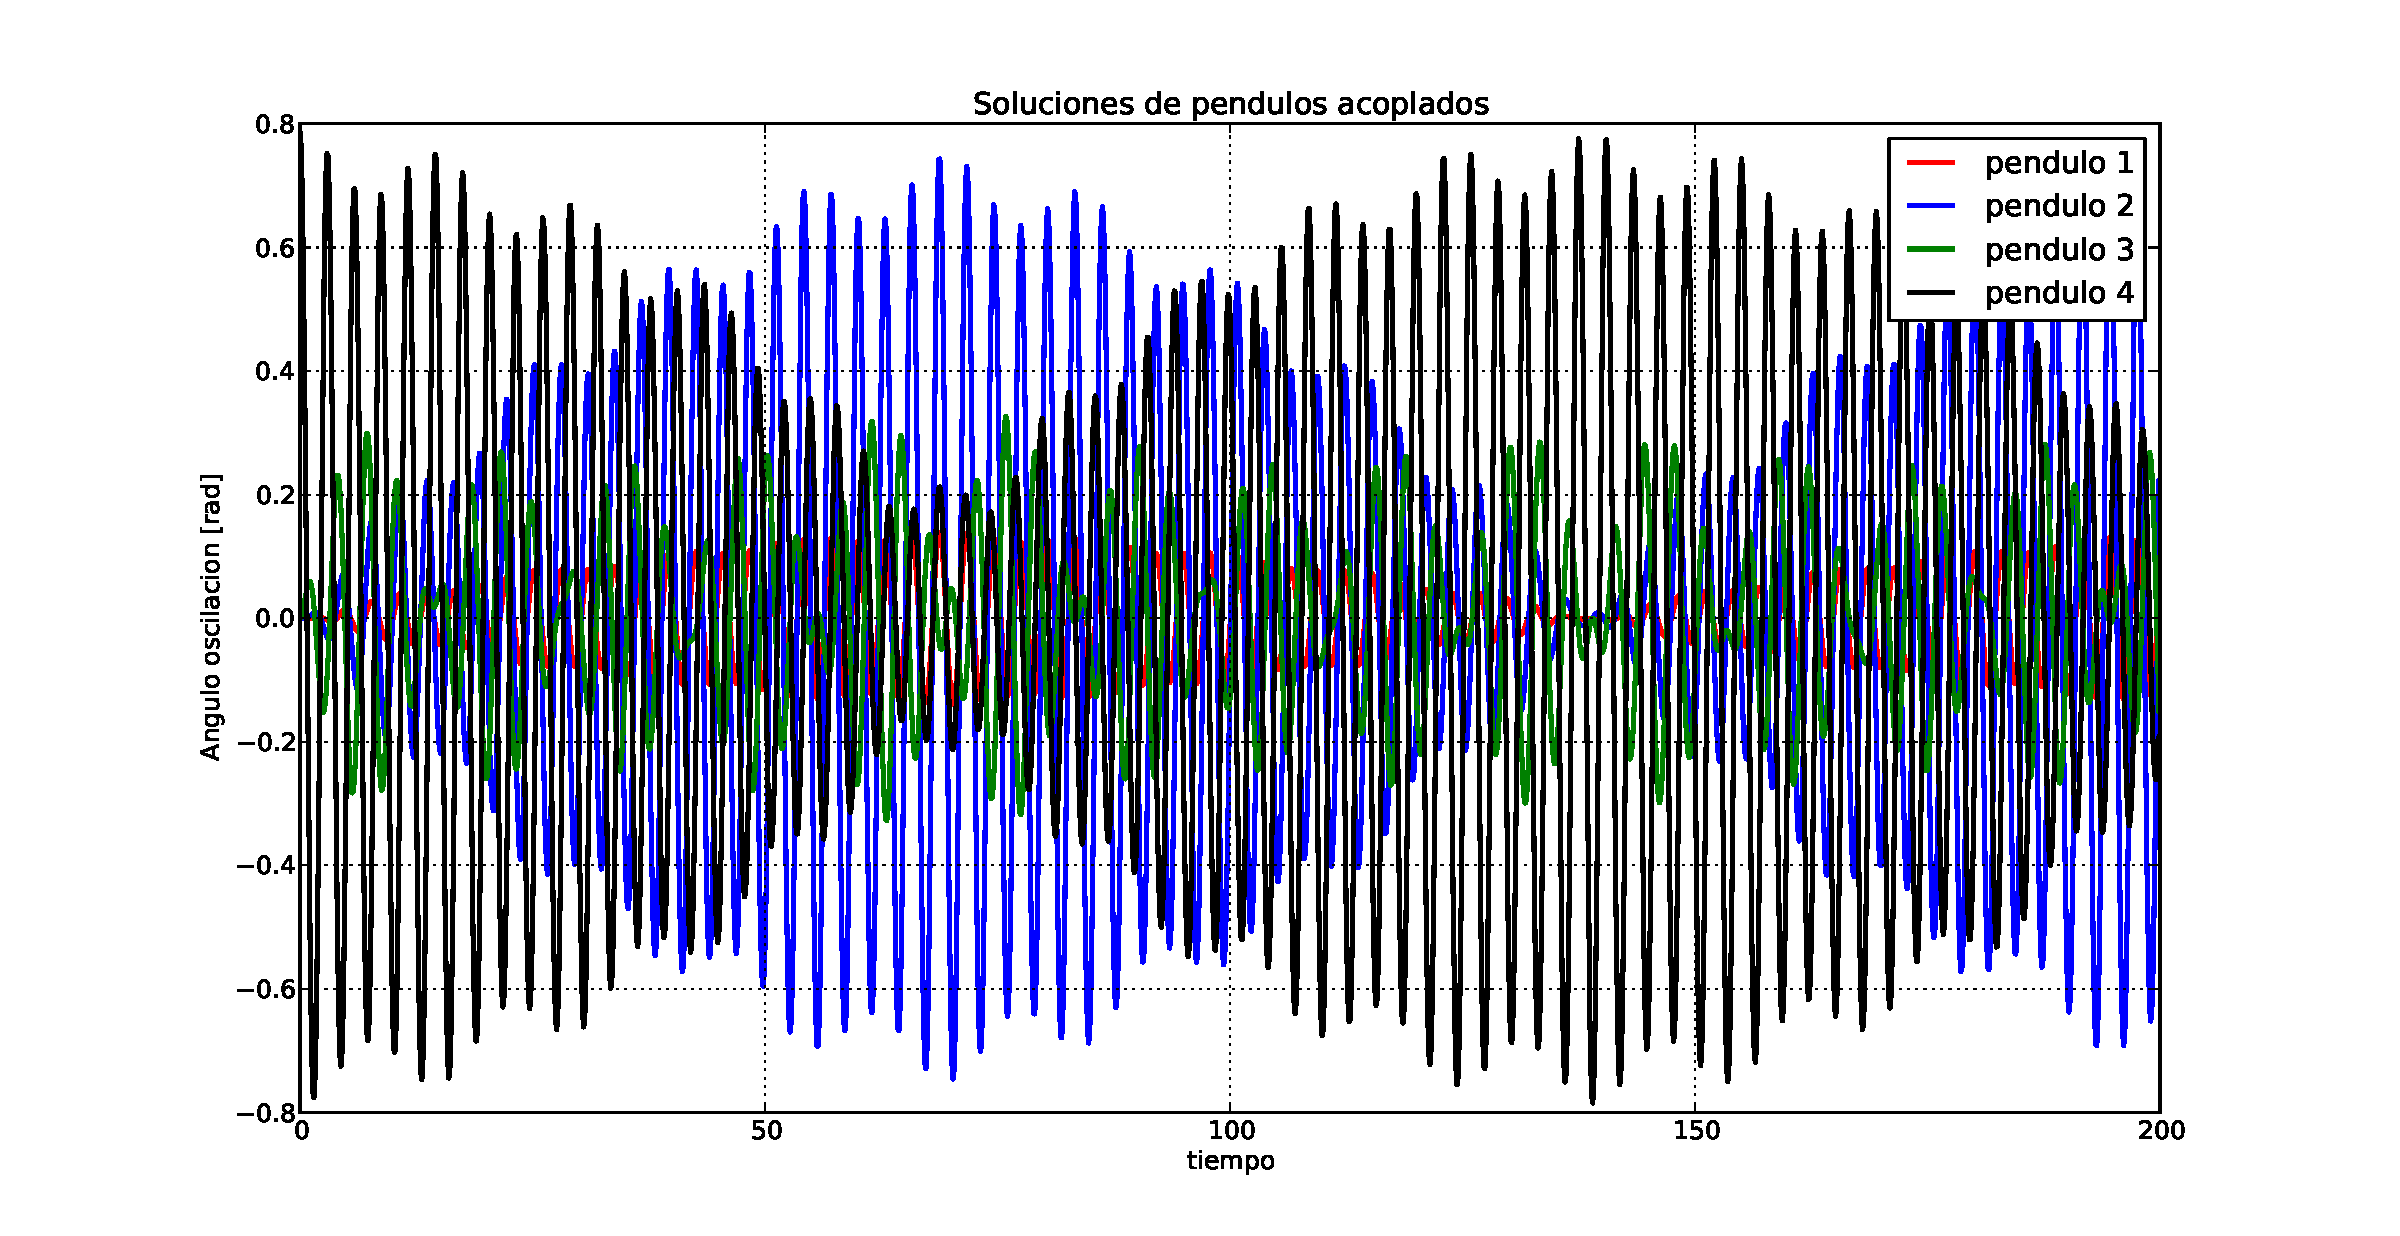
\includegraphics[width=1.0\textwidth]
	{./pictures/demo2_03(02).pdf}

	\caption{\small{Solución de la amplitud para cada uno de los cuatro 
	péndulos acoplados del sistema. Puede notarse que a pesar de que los
	péndulos 1 y 3 comienzan a oscilar, absorbiendo parte de la energía 
	del péndulo 4, el péndulo 2 lo hace más eficientemente debido a tener 
	la misma longitud, presentando resonancia.}}
	
	\label{fig:four_pedulum}
\end{figure}
%.........................................................................


A continuación se explica el código anterior

%ccccccccccccccccccccccccccccccccccccccccccccccccccccccccccccccccccccccccc
%DEMO 2_03
\begin{listing}[style=python, numbers = none]
from __future__ import division
import numpy as np
import matplotlib.pylab as plt
import scipy.integrate as integ
\end{listing}
%ccccccccccccccccccccccccccccccccccccccccccccccccccccccccccccccccccccccccc
La primera línea hace que \python divida entre enteros de forma adecuada 
ya que por defecto cuando se dividen dos enteros se retorna el residuo entero
entre la división, por ejemplo sin la primera línea \texttt{3/2 = 1}, 
y con ella, \texttt{3/2 = 1.5}. Se recomienda siempre usarla. Las demás
lineas corresponden a las librerías ya conocidas importadas bajo los alias
estándares.


%ccccccccccccccccccccccccccccccccccccccccccccccccccccccccccccccccccccccccc
%DEMO 2_03
\begin{listing}[style=python, numbers = none]
#Guardado de resultados en archivo externo
datos = np.transpose((tiempo, theta1_t, theta2_t, \
theta3_t, theta4_t))
np.savetxt( 'amplitudes.txt', datos )
\end{listing}
%ccccccccccccccccccccccccccccccccccccccccccccccccccccccccccccccccccccccccc
En la primera línea se crea un arreglo con las diferentes columnas del 
archivo que se desea guardar, en este caso es el arreglo de tiempo en la 
primera y los arreglos con la solución de los ángulos para los 4 péndulos
en las siguientes. El operador backslash $\backslash$ permite saltar de línea 
en \python sin que haya problemas de sintaxis y sirve para organizar el 
código y hacerlo más legible. La función de \numpy \texttt{transpose} se 
usa para transponer la matriz (arreglo) de datos para que el archivo 
externo esté organizado por columnas y no por filas. Finalmente la función
\texttt{savetxt} permite guardar todos los datos en un archivo externo 
llamado \texttt{amplitudes.txt}.


%ccccccccccccccccccccccccccccccccccccccccccccccccccccccccccccccccccccccccc
%DEMO 2_03
\begin{listing}[style=python, numbers = none]
#Grafica de las soluciones
plt.plot( tiempo, theta1_t, label = 'pendulo 1', \
color='red', linewidth = 2 )
plt.plot( tiempo, theta2_t, label = 'pendulo 2', \
color='blue', linewidth = 2 )
plt.plot( tiempo, theta3_t, label = 'pendulo 3', \
color='green', linewidth = 2 )
plt.plot( tiempo, theta4_t, label = 'pendulo 4', \
color='black', linewidth = 2 )
\end{listing}
%ccccccccccccccccccccccccccccccccccccccccccccccccccccccccccccccccccccccccc
En esta parte se grafican en una misma ventana todas las soluciones para 
los 4 péndulos. Se usa de nuevo el operador backslash $\backslash$ para
ordenar el código y se aplican nuevos argumentos de la función 
\texttt{plot} de la librería \matplotlib. El argumento \texttt{color} 
permite definir el color de la curva mientras que \texttt{linewidth}
define el grosor, el valor de \texttt{1} se toma por defecto si no se 
especifica.


%ccccccccccccccccccccccccccccccccccccccccccccccccccccccccccccccccccccccccc
%DEMO 2_03
\begin{listing}[style=python, numbers = none]
#Formato de grafica
plt.title('Soluciones de pendulos acoplados')
plt.xlabel('tiempo')
plt.ylabel('Angulo oscilacion [rad]')
plt.grid()
plt.legend()
plt.show()
\end{listing}
%ccccccccccccccccccccccccccccccccccccccccccccccccccccccccccccccccccccccccc
En esta última parte se usan funciones de \matplotlib para dar formato a 
las gráficas. En primer lugar se asigna un título con la función 
\texttt{title}, luego se asignan etiquetas en cada eje con las funciones 
\texttt{xlabel} y \texttt{ylabel}, se activa una malla sobre la ventana 
con la función \texttt{grid} y finalmente se muestran las etiquetas de 
cada curva con \texttt{legend} y se muestra el resultado en pantalla con
\texttt{show}.

\

\

Como segunda parte de esta demostración se usaran los datos integrados 
y almacenados en el archivo \texttt{amplitudes.txt} para representar una 
animación 3D del sistema.


\rule{14cm}{0.5mm}
%*************************************************************************
